% GHOST overview infographic. Designed at 7.16in = IEEE \textwidth.
\documentclass[tikz,border=2pt,9pt]{standalone}
\usepackage[T1]{fontenc}
\usepackage{mathptmx}
\usepackage{amsmath,amssymb}
\usetikzlibrary{arrows.meta,calc,positioning,shapes.misc}
\definecolor{navy}{HTML}{011E4B}
\definecolor{gold}{HTML}{FAB001}
\definecolor{sky}{HTML}{87C6E9}
\definecolor{alert}{HTML}{EE1C23}
\definecolor{skyd}{HTML}{3A8FC6}

\tikzset{
  >={Stealth[length=1.8mm,width=1.4mm]},
  panel/.style={draw=navy,line width=0.7pt,fill=white,rounded corners=2.5pt},
  ptitle/.style={font=\bfseries\small,text=navy,anchor=west,inner sep=0pt},
  blk/.style={draw=navy,line width=0.5pt,fill=white,rounded corners=1.5pt,inner sep=2pt,align=center,font=\scriptsize,text=navy},
  blkt/.style={font=\scriptsize\bfseries,text=navy,inner sep=0pt,anchor=south},
  capt/.style={font=\tiny\itshape,text=skyd,inner sep=0pt,align=center},
  note/.style={font=\tiny,text=navy,inner sep=0pt,align=center},
  flow/.style={->,draw=navy,line width=0.7pt},
  sflow/.style={->,draw=sky,line width=1.5pt},
  pill/.style={fill=navy,text=white,font=\tiny\bfseries,rounded corners=2.5mm,inner xsep=5pt,inner ysep=2.5pt},
  gpill/.style={fill=gold,text=navy,font=\tiny\bfseries,rounded corners=2.5mm,inner xsep=5pt,inner ysep=2.5pt},
  rpill/.style={fill=alert,text=white,font=\tiny\bfseries,rounded corners=2.5mm,inner xsep=5pt,inner ysep=2.5pt},
  num/.style={circle,fill=navy,text=white,font=\tiny\bfseries,inner sep=0pt,minimum size=3.6mm},
}
% ---------------------------------------------------------------- icons
\newcommand{\tile}[4]{%
\begin{scope}[shift={(#1,#2)}]
  \pgfmathsetseed{#3}
  \foreach \i in {0,1,2}{\foreach \j in {0,1,2}{
    \pgfmathsetmacro{\v}{int(25+random()*70)}
    \fill[#4!\v!white] (\i*0.11,\j*0.11) rectangle ++(0.11,0.11);}}
  \draw[navy,line width=0.3pt] (0,0) rectangle (0.33,0.33);
\end{scope}}
\newcommand{\dtile}[3]{%
\begin{scope}[shift={(#1,#2)}]
  \pgfmathsetseed{#3}
  \foreach \i in {0,1,2}{\foreach \j in {0,1,2}{
    \pgfmathsetmacro{\v}{int(20+random()*60)}
    \fill[gold!\v!white] (\i*0.11,\j*0.11) rectangle ++(0.11,0.11);}}
  \draw[navy,line width=0.4pt,densely dashed] (0,0) rectangle (0.33,0.33);
\end{scope}}
\newcommand{\fmap}[5]{%
\begin{scope}[shift={(#1,#2)}]
  \pgfmathsetseed{#3}
  \foreach \i in {0,1,2,3,4}{\foreach \j in {0,1,2,3,4}{
    \pgfmathsetmacro{\s}{100*(1-#5)*(0.25+0.5*abs(sin(60*\i+40*\j)))+100*#5*random()}
    \pgfmathsetmacro{\v}{int(\s)}
    \fill[#4!\v!white] (\i*0.1,\j*0.1) rectangle ++(0.1,0.1);}}
  \draw[navy,line width=0.3pt] (0,0) rectangle (0.5,0.5);
\end{scope}}
\newcommand{\padlock}[4]{%
\begin{scope}[shift={(#1,#2)}]
  \fill[#3,rounded corners=0.6pt] (-0.16,-0.17) rectangle (0.16,0.05);
  \ifnum#4=0 \draw[#3,line width=1.3pt] (-0.09,0.05) -- (-0.09,0.15) arc (180:0:0.09) -- (0.09,0.05);
  \else \draw[#3,line width=1.3pt] (-0.09,0.05) -- (-0.09,0.15) arc (180:0:0.09) -- (0.09,0.11);\fi
  \fill[white] (0,-0.06) circle (0.03);
\end{scope}}
\newcommand{\cloud}[3]{%
\begin{scope}[shift={(#1,#2)},scale=#3]
  \fill[sky] (0,0) circle (0.22) (0.28,0.05) circle (0.18) (-0.26,0.02) circle (0.16) (0.05,-0.12) ellipse (0.5 and 0.16);
\end{scope}}
\newcommand{\token}[2]{%
\begin{scope}[shift={(#1,#2)}]
  \fill[gold] (0,0) circle (0.16); \draw[navy,line width=0.6pt] (0,0) circle (0.16);
  \node[font=\tiny\bfseries,text=navy] at (0,0) {$\tau$};
\end{scope}}
\newcommand{\eye}[2]{%
\begin{scope}[shift={(#1,#2)}]
  \draw[alert,line width=0.8pt] (-0.2,0) .. controls (-0.08,0.16) and (0.08,0.16) .. (0.2,0) .. controls (0.08,-0.16) and (-0.08,-0.16) .. (-0.2,0);
  \fill[alert] (0,0) circle (0.06);
\end{scope}}
\newcommand{\meter}[6]{%
  \draw[navy,line width=0.4pt] (#1,#2) rectangle ++(#3,0.17);
  \fill[#5] (#1+0.02,#2+0.02) rectangle ++({(#3-0.04)*#4},0.13);
  \node[font=\tiny\bfseries,text=navy,anchor=west,inner sep=0pt] at (#1+#3+0.07,#2+0.085) {#6};}

\begin{document}
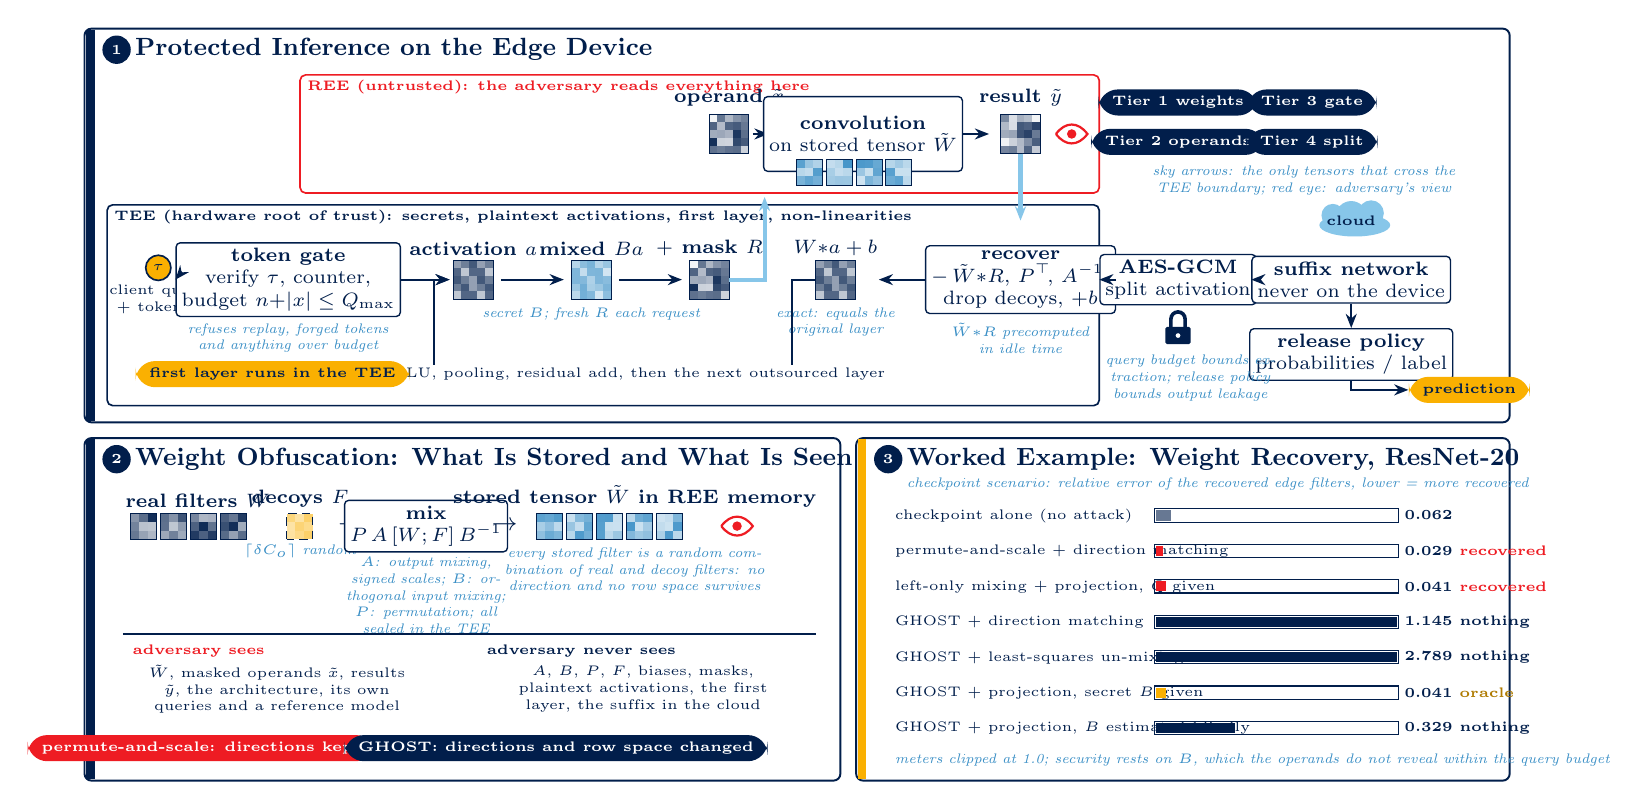
\begin{tikzpicture}[x=1cm,y=1cm]
%% ================================================================== PANEL 1
\node[panel,minimum width=18.1cm,minimum height=5.0cm,anchor=north west] (P1) at (0,0) {};
\fill[navy] ($(P1.north west)+(0.03,-0.03)$) rectangle ($(P1.south west)+(0.14,0.03)$);
\node[num] at (0.42,-0.28) {1};
\node[ptitle] at (0.65,-0.28) {Protected Inference on the Edge Device};

\draw[alert,line width=0.6pt,rounded corners=2pt] (2.75,-0.6) rectangle (12.9,-2.1);
\node[font=\tiny\bfseries,text=alert,anchor=north west,inner sep=1pt] at (2.8,-0.62) {REE (untrusted): the adversary reads everything here};
\draw[navy,line width=0.6pt,rounded corners=2pt] (0.3,-2.25) rectangle (12.9,-4.8);
\node[font=\tiny\bfseries,text=navy,anchor=north west,inner sep=1pt] at (0.35,-2.27) {TEE (hardware root of trust): secrets, plaintext activations, first layer, non-linearities};

\token{0.95}{-3.05}
\node[note] at (0.95,-3.45) {client query\\$+$ token $\tau$};
\node[blk,minimum width=1.6cm] (gate) at (2.6,-3.2) {\textbf{token gate}\\verify $\tau$, counter,\\budget $n{+}|x|\le Q_{\max}$};
\draw[flow] (1.25,-3.1) -- (gate.west);
\node[capt,anchor=north] at (2.6,-3.75) {refuses replay, forged tokens\\and anything over budget};

\node[blkt] at (4.95,-2.9) {activation $a$};
\fmap{4.7}{-3.45}{3}{navy}{0}
\draw[flow] (5.3,-3.2) -- (6.1,-3.2);
\node[blkt] at (6.45,-2.9) {mixed $Ba$};
\fmap{6.2}{-3.45}{7}{skyd}{0.15}
\draw[flow] (6.8,-3.2) -- (7.6,-3.2);
\node[blkt] at (7.95,-2.9) {$+$ mask $R$};
\fmap{7.7}{-3.45}{11}{navy}{0.95}
\node[capt,anchor=north] at (6.45,-3.55) {secret $B$; fresh $R$ each request};

\draw[sflow] (8.2,-3.2) -- (8.65,-3.2) -- (8.65,-2.15);
\node[blkt] at (8.2,-1.0) {operand $\tilde x$};
\fmap{7.95}{-1.6}{11}{navy}{0.95}
\draw[flow] (8.5,-1.35) -- (8.7,-1.35);
\node[blk,minimum width=2.3cm,minimum height=0.95cm] (conv) at (9.9,-1.35) {\textbf{convolution}\\on stored tensor $\tilde W$};
\tile{9.05}{-2.0}{21}{skyd}\tile{9.43}{-2.0}{22}{skyd}\tile{9.81}{-2.0}{23}{skyd}\tile{10.19}{-2.0}{24}{skyd}
\draw[flow] (conv.east) -- (11.5,-1.35);
\node[blkt] at (11.9,-1.0) {result $\tilde y$};
\fmap{11.65}{-1.6}{31}{navy}{0.9}
\eye{12.55}{-1.35}
\draw[sflow] (11.9,-1.6) -- (11.9,-2.45);
\node[blk,minimum width=1.9cm] (rec) at (11.9,-3.2) {\textbf{recover}\\$-\,\tilde W{*}R$, $P^{\top}\!$, $A^{-1}$,\\drop decoys, $+b$};
\node[capt,anchor=north] at (11.9,-3.75) {$\tilde W{*}R$ precomputed\\in idle time};
\draw[flow] (rec.west) -- (10.1,-3.2);
\node[blkt] at (9.55,-2.9) {$W{*}a+b$};
\fmap{9.3}{-3.45}{41}{navy}{0}
\node[capt,anchor=north] at (9.55,-3.55) {exact: equals the\\original layer};
\draw[flow] (9.3,-3.2) -- (9.0,-3.2) -- (9.0,-4.4) -- (4.45,-4.4) -- (4.45,-3.2) -- (4.65,-3.2);
\node[note,fill=white,inner sep=1pt] at (7.0,-4.4) {ReLU, pooling, residual add, then the next outsourced layer};
\node[gpill] at (2.4,-4.4) {first layer runs in the TEE};
\draw[flow] (gate.east) -- (4.65,-3.2);

\node[blk,minimum width=1.5cm] (aes) at (13.9,-3.2) {\textbf{AES-GCM}\\split activation};
\draw[flow] (rec.east) -- (aes.west);
\padlock{13.9}{-3.85}{navy}{0}
\cloud{16.1}{-2.4}{0.9}
\node[font=\tiny\bfseries,text=navy] at (16.1,-2.45) {cloud};
\node[blk,minimum width=1.9cm] (suf) at (16.1,-3.2) {\textbf{suffix network}\\never on the device};
\node[blk,minimum width=1.9cm] (pol) at (16.1,-4.15) {\textbf{release policy}\\probabilities / label};
\draw[flow] (aes.east) -- (suf.west);
\draw[flow] (suf) -- (pol);
\node[gpill] (pred) at (17.6,-4.6) {prediction};

\draw[flow] (pol.south) -- (16.1,-4.6) -- (pred.west);
\node[capt,anchor=west,text width=2.2cm] at (12.95,-4.45) {query budget bounds extraction; release policy bounds output leakage};

\node[pill] at (13.9,-0.95) {Tier 1 weights};
\node[pill] at (13.9,-1.45) {Tier 2 operands};
\node[pill] at (15.6,-0.95) {Tier 3 gate};
\node[pill] at (15.6,-1.45) {Tier 4 split};
\node[capt,anchor=north,text width=4.4cm] at (15.5,-1.75) {sky arrows: the only tensors that cross the TEE boundary; red eye: adversary's view};

%% ================================================================== PANEL 2
\node[panel,minimum width=9.6cm,minimum height=4.35cm,anchor=north west] (P2) at (0,-5.2) {};
\fill[navy] ($(P2.north west)+(0.03,-0.03)$) rectangle ($(P2.south west)+(0.14,0.03)$);
\node[num] at (0.42,-5.48) {2};
\node[ptitle] at (0.65,-5.48) {Weight Obfuscation: What Is Stored and What Is Seen};

\node[blkt] at (1.45,-6.1) {real filters $W$};
\tile{0.6}{-6.5}{51}{navy}\tile{0.98}{-6.5}{52}{navy}\tile{1.36}{-6.5}{53}{navy}\tile{1.74}{-6.5}{54}{navy}
\node[blkt] at (2.75,-6.1) {decoys $F$};
\dtile{2.58}{-6.5}{55}
\node[capt,anchor=north] at (2.75,-6.55) {$\lceil\delta C_o\rceil$ random};
\node[font=\small,text=navy] at (3.4,-6.33) {$\rightarrow$};
\node[blk,minimum width=1.5cm] (mix) at (4.35,-6.33) {\textbf{mix}\\$P\,A\,[W;F]\,B^{-1}$};
\node[capt,anchor=north,text width=2.4cm] at (4.35,-6.72) {$A$: output mixing, signed scales; $B$: orthogonal input mixing; $P$: permutation; all sealed in the TEE};
\node[font=\small,text=navy] at (5.35,-6.33) {$\rightarrow$};
\node[blkt] at (7.0,-6.1) {stored tensor $\tilde W$ in REE memory};
\tile{5.75}{-6.5}{61}{skyd}\tile{6.13}{-6.5}{62}{skyd}\tile{6.51}{-6.5}{63}{skyd}\tile{6.89}{-6.5}{64}{skyd}\tile{7.27}{-6.5}{65}{skyd}
\eye{8.3}{-6.33}
\node[capt,anchor=north,text width=3.6cm] at (7.0,-6.6) {every stored filter is a random combination of real and decoy filters: no direction and no row space survives};

\draw[navy,line width=0.4pt] (0.5,-7.7) -- (9.3,-7.7);
\node[font=\tiny\bfseries,text=alert,anchor=west] at (0.5,-7.92) {adversary sees};
\node[note,anchor=west,text width=3.9cm] at (0.5,-8.4) {$\tilde W$, masked operands $\tilde x$, results $\tilde y$, the architecture, its own queries and a reference model};
\node[font=\tiny\bfseries,text=navy,anchor=west] at (5.0,-7.92) {adversary never sees};
\node[note,anchor=west,text width=4.2cm] at (5.0,-8.4) {$A$, $B$, $P$, $F$, biases, masks, plaintext activations, the first layer, the suffix in the cloud};
\node[rpill] at (1.5,-9.15) {permute-and-scale: directions kept};
\node[pill] at (6.0,-9.15) {GHOST: directions and row space changed};

%% ================================================================== PANEL 3
\node[panel,minimum width=8.3cm,minimum height=4.35cm,anchor=north west] (P3) at (9.8,-5.2) {};
\fill[gold] ($(P3.north west)+(0.03,-0.03)$) rectangle ($(P3.south west)+(0.14,0.03)$);
\node[num] at (10.22,-5.48) {3};
\node[ptitle] at (10.45,-5.48) {Worked Example: Weight Recovery, ResNet-20};
\node[capt,anchor=west] at (10.45,-5.8) {checkpoint scenario: relative error of the recovered edge filters, lower = more recovered};

\def\mx{3.1}
\node[note,anchor=west] at (10.3,-6.2) {checkpoint alone (no attack)};
\meter{13.6}{-6.28}{\mx}{0.062}{navy!60!white}{0.062}
\node[note,anchor=west] at (10.3,-6.65) {permute-and-scale $+$ direction matching};
\meter{13.6}{-6.73}{\mx}{0.029}{alert}{0.029 \textcolor{alert}{recovered}}
\node[note,anchor=west] at (10.3,-7.1) {left-only mixing $+$ projection, $Q$ given};
\meter{13.6}{-7.18}{\mx}{0.041}{alert}{0.041 \textcolor{alert}{recovered}}
\node[note,anchor=west] at (10.3,-7.55) {GHOST $+$ direction matching};
\meter{13.6}{-7.63}{\mx}{1.0}{navy}{1.145 \textcolor{navy}{nothing}}
\node[note,anchor=west] at (10.3,-8.0) {GHOST $+$ least-squares un-mixing};
\meter{13.6}{-8.08}{\mx}{1.0}{navy}{2.789 \textcolor{navy}{nothing}}
\node[note,anchor=west] at (10.3,-8.45) {GHOST $+$ projection, secret $B$ given};
\meter{13.6}{-8.53}{\mx}{0.041}{gold}{0.041 \textcolor{gold!70!black}{oracle}}
\node[note,anchor=west] at (10.3,-8.9) {GHOST $+$ projection, $B$ estimated blindly};
\meter{13.6}{-8.98}{\mx}{0.33}{navy}{0.329 \textcolor{navy}{nothing}};
\node[capt,anchor=west] at (10.3,-9.3) {meters clipped at 1.0; security rests on $B$, which the operands do not reveal within the query budget};
\end{tikzpicture}
\end{document}
